%%%%%%%%%%%%%%%%%%%%%%%%%%%%%%%%%%%%%%%%%
% Jacobs Portrait Poster
% LaTeX Template
% Version 1.0 (31/08/2015)
% (Based on Version 1.0 (29/03/13) of the landscape template
%
% Created by:
% Computational Physics and Biophysics Group, Jacobs University
% https://teamwork.jacobs-university.de:8443/confluence/display/CoPandBiG/LaTeX+Poster
% 
% Further modified by:
% Nathaniel Johnston (nathaniel@njohnston.ca)
%
% Portrait version by:
% John Hammersley
%
% The landscape version of this template was downloaded from:
% http://www.LaTeXTemplates.com
%
% License:
% CC BY-NC-SA 3.0 (http://creativecommons.org/licenses/by-nc-sa/3.0/)
%
%%%%%%%%%%%%%%%%%%%%%%%%%%%%%%%%%%%%%%%%%

%----------------------------------------------------------------------------------------
%	PACKAGES AND OTHER DOCUMENT CONFIGURATIONS
%----------------------------------------------------------------------------------------

\documentclass[final]{beamer}

\usepackage[utf8]{inputenc}

\usepackage[scale=1.4]{beamerposter} % Use the beamerposter package for laying out the poster

\usetheme{confposter} % Use the confposter theme supplied with this template

\setbeamercolor{block title}{fg=unipeAzul,bg=unipeCeleste!10} % Colors of the block titles
\setbeamercolor{block body}{fg=unipeAzul,bg=white} % Colors of the body of blocks
\setbeamercolor{block alerted title}{fg=white,bg=unipeVioleta} % Colors of the highlighted block titles
\setbeamercolor{block alerted body}{fg=black,bg=unipeVioleta!10} % Colors of the body of highlighted blocks
\setbeamercolor{item}{fg=unipeVioleta}
\setbeamercolor{item projected}{bg=unipeVioleta, fg=white}
% Many more colors are available for use in beamerthemeconfposter.sty

%-----------------------------------------------------------
% Define the column widths and overall poster size
% To set effective sepwid, onecolwid and twocolwid values, first choose how many columns you want and how much separation you want between columns
% In this template, the separation width chosen is 0.024 of the paper width and a 4-column layout
% onecolwid should therefore be (1-(# of columns+1)*sepwid)/# of columns e.g. (1-(4+1)*0.024)/4 = 0.22
% Set twocolwid to be (2*onecolwid)+sepwid = 0.464
% Set threecolwid to be (3*onecolwid)+2*sepwid = 0.708

\newlength{\sepwid}
\newlength{\onecolwid}
\newlength{\twocolwid}
\newlength{\threecolwid}
\setlength{\paperwidth}{36in} % A0 width: 46.8in
\setlength{\paperheight}{48in} % A0 height: 33.1in
\setlength{\sepwid}{0.024\paperwidth} % Separation width (white space) between columns
\setlength{\onecolwid}{0.22\paperwidth} % Width of one column
\setlength{\twocolwid}{0.44\paperwidth} % Width of two columns
\setlength{\threecolwid}{0.708\paperwidth} % Width of three columns
\setlength{\topmargin}{-0.5in} % Reduce the top margin size
%-----------------------------------------------------------

\usepackage{graphicx}  % Required for including images

\usepackage{booktabs} % Top and bottom rules for tables

%----------------------------------------------------------------------------------------
%	TITLE SECTION 
%----------------------------------------------------------------------------------------

\title{Zamba: una plataforma de aprendizaje como soporte a conceptos computacionales} % Poster title

\author{Gustavo del Dago (gustavo.deldago@unipe.edu.ar), Virginia Brassesco(virginia.brassesco@unipe.edu.ar) y Maximiliano Urso(maximiliano.urso@unipe.edu.ar)}
% Author(s)

\institute{Universidad Pedagógica Nacional} % Institution(s)

%----------------------------------------------------------------------------------------

\begin{document}

\addtobeamertemplate{block end}{}{\vspace*{2ex}} % White space under blocks
\addtobeamertemplate{block alerted end}{}{\vspace*{2ex}} % White space under highlighted (alert) blocks

\setlength{\belowcaptionskip}{2ex} % White space under figures
\setlength\belowdisplayshortskip{2ex} % White space under equations

\begin{frame}[t] % The whole poster is enclosed in one beamer frame

\begin{columns}[t] % The whole poster consists of three major columns, the second of which is split into two columns twice - the [t] option aligns each column's content to the top

\begin{column}{\sepwid}\end{column} % Empty spacer column

\begin{column}{\twocolwid} % The first column

%----------------------------------------------------------------------------------------
%	OBJECTIVES
%----------------------------------------------------------------------------------------

\begin{alertblock}{Objetivos}
    \begin{itemize}
        \item Tener una plataforma en español y personalizable, para curso introductoria de programación por bloques con entorno minimalista y sin instalación
        \item Tener una herramienta que permita la transición a lenguajes textuales
        \item Plataforma didáctica como soporte para estrategias didácticas
        \item Enseñar conceptos de  variables, entrada y salida utilizando bloques y tipos de datos básicos (Cadenas de texto, Números, Lógicos)
    \end{itemize}
\end{alertblock}

%----------------------------------------------------------------------------------------
%	INTRODUCTION
%----------------------------------------------------------------------------------------

\begin{block}{Motivación}
    La UniPe está diseñando un Profesorado en Informática innovador, alineado con los aprendizajes del Programa Nacional de Ciencia y Tecnología en la Escuela del MinCyT.
    El objetivo de la materia de Programación 1 se centra en poder pensar estrategias simples centradas en la legibilidad de código. 
    Los desafíos son algoritmos de recorridos secuenciales.
\end{block}

\begin{figure}
	\centering
	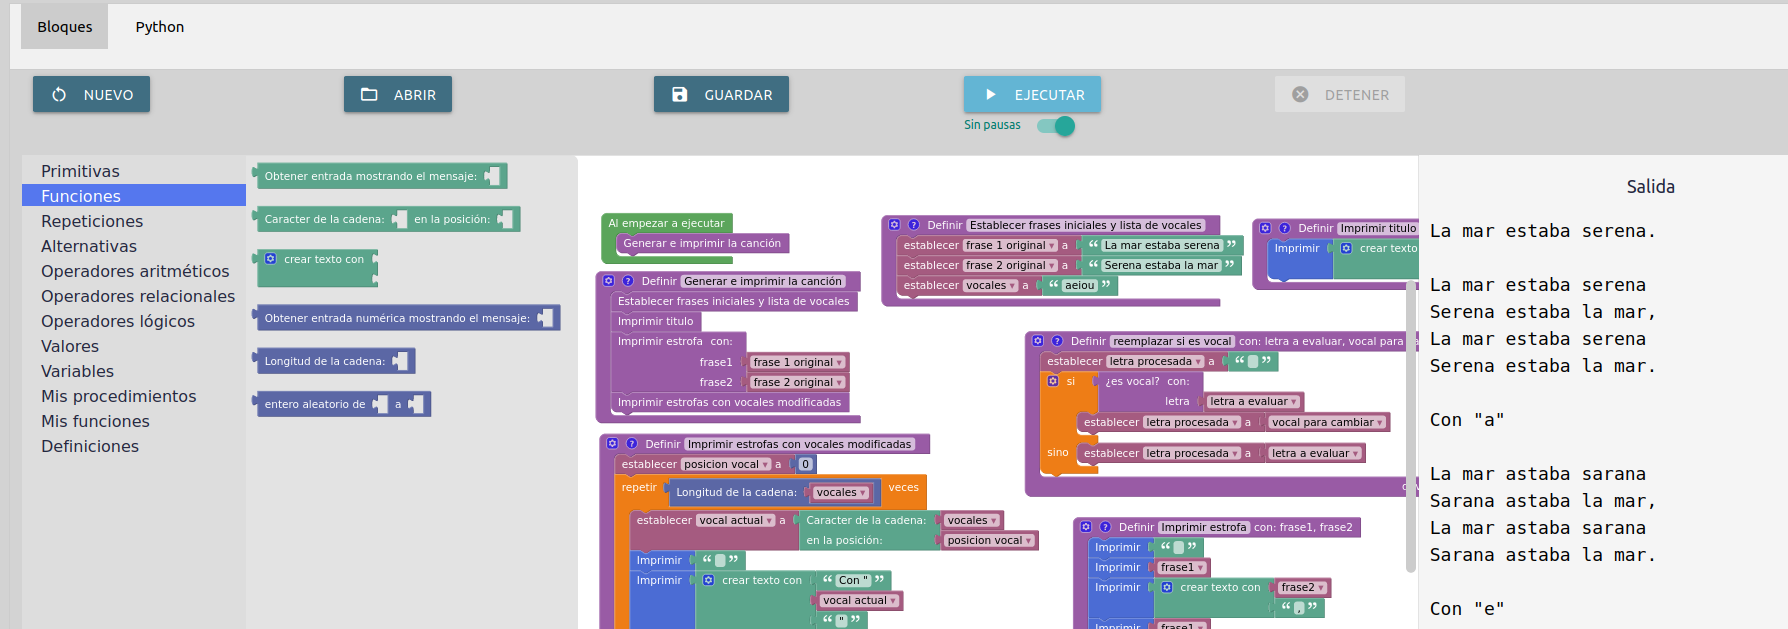
\includegraphics[width=1\linewidth]{zamba}
	\caption{Entorno Zamba}
	\label{fig:zamba}
\end{figure}

\begin{figure}
	\centering
	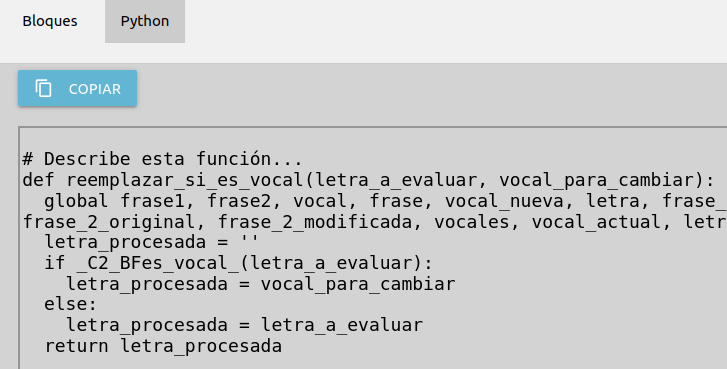
\includegraphics[width=0.7\linewidth]{pythonzamba.png}
	\caption{Traducción a Python automática}
	\label{fig:traduccion}
\end{figure}

\begin{block}{Desventajas de entornos existentes}
\begin{itemize}
    \item Idioma, no tienen todos los bloques traducidos, o las palabras no son Argentinas.
    \item Más estructuras y conceptos computacionales del mínimo requerido para resolver
    \item Requieren registro
    \item Entornos más pesados gráficamente
    %\item Colores de estructuras distintos a los usados en Pilas Bloques
\end{itemize}
\end{block}


%------------------------------------------------



%----------------------------------------------------------------------------------------

\end{column} % End of the first column

\begin{column}{\sepwid}\end{column} % Empty spacer column  

\begin{column}{\sepwid}\end{column} % Empty spacer column

\begin{column}{\twocolwid} % The third column


\begin{block}{Ventajas de diseñar entorno propio}
\begin{itemize}
    \item Construye ``Soberanía Pedagógica''
    \item División y nombre de categorías propia, basada en bibliografía de la materia
    \item Readecuación de herramienta durante la cursada basada en la necesidad del estudiantado
    \item Incentivar al diseño de las propias herramientas como soporte a conceptos
    \item Permite el pasaje a lenguaje de programación textual
    \item Basado en Blockly\cite{blockly} con mucha documentación y experiencias alrededor del mundo
\end{itemize}


\end{block}

\begin{block}{Construcción y Diseño}
    \begin{enumerate}
        \item Diseño de unidades didácticas y sus guías de ejercicios
        \item En cada ejercicio anotar los conceptos algorítmicos y estructuras computacionales requeridas
        \item Armar la paleta de conceptos computacionales con los requerimientos de los ejercicios
        \item Adecuación de Blockly\cite{blockly} con pausas y traducción a Python 
        \item Montado en GitHub Pages

    \end{enumerate}

\end{block}

%----------------------------------------------------------------------------------------
%	CONCLUSION
%----------------------------------------------------------------------------------------

% \begin{block}{Trabajo a futuro}
% Nos gustaría entender si:
%     \begin{itemize}
%         \item Zamba cubre con su funcionalidad los conceptos fundamentales que se dictan en el curso. Por ej: Repetición condicional, modularización, interactividad, flujo de información en un programa.
%         \item Estudiantes que usan Pilas Bloques encuentran las nuevas funciones indagando
%         \item Cómo reaccionan los alumnos que tienen experiencia previa programando
%     \end{itemize}
% \end{block}

\begin{block}{Conclusiones}
    \begin{itemize}
        \item Es una herramienta modificable con facilidad. Se puede descargar y usar de forma gratuita y desconectada en cualquier navegador.
        \item Al estar basado en Blockly, cuenta con la herramienta de traducción a lenguajes de texto, personalizable
        \item Las variables en Zamba son todas globales, esto permite un debate amplio de alcance de las variables y flujo de información al enfrentarse a otros lenguajes donde esto es más restringido.
        \item Una contra es que permite programar procedimientos con efectos colaterales sobre las variables, al no controlar estrictamente el flujo de información los programas pueden tener resultados no deseados.
        \item Se deben reforzar los conceptos de creación, inicialización y asignación de variables en el código como concepto principal para asegurar precondiciones de valores válidos en las rutinas.
    \end{itemize}
\end{block}

\begin{block}{Referencias}

\nocite{*} % Insert publications even if they are not cited in the poster
\small{\bibliographystyle{unsrt}
\bibliography{sample}\vspace{0.75in}}

\end{block}


%----------------------------------------------------------------------------------------
%	ADDITIONAL INFORMATION
%----------------------------------------------------------------------------------------


%----------------------------------------------------------------------------------------

\end{column} % End of the third column

\end{columns} % End of all the columns in the poster

\end{frame} % End of the enclosing frame

\end{document}
